%%%%%%%%%%%%%%%%%%%%%%%%%%%%%%%%%%%%%%%%%%%%%%%%%%%%%%%%%%%%%%%%%%%%%%%%%%%%%%%%
% IEEE Conference Format Research Paper
% Title: ForgeSight AI: An Explainable Federated Digital Twin Framework for Predictive Maintenance in Smart Manufacturing
% Authors: Mr. Shubham Utekar, Dr. Santosh Rane
%%%%%%%%%%%%%%%%%%%%%%%%%%%%%%%%%%%%%%%%%%%%%%%%%%%%%%%%%%%%%%%%%%%%%%%%%%%%%%%%

\documentclass[letterpaper, 10 pt, conference]{ieeeconf}

\IEEEoverridecommandlockouts
\overrideIEEEmargins

\usepackage[utf8]{inputenc}
\usepackage[T1]{fontenc}
\usepackage{graphicx}
\usepackage{amsmath}
\usepackage{amssymb}
\usepackage{array}
\usepackage{booktabs}
\usepackage{multirow}
\usepackage{url}
\usepackage{cite}
\usepackage{tikz}
\usepackage{pgfplots}
\usepackage{algorithm}
\usepackage{algorithmic}
\usetikzlibrary{arrows.meta, positioning, shapes.geometric, shapes.multipart, fit, calc}
\pgfplotsset{compat=1.15}

\title{\LARGE \bf
ForgeSight AI: An Explainable Federated Digital Twin Framework for Predictive Maintenance in Smart Manufacturing
}

\author{
\begin{tabular}{cc}
\begin{minipage}{0.45\textwidth}
\centering
Mr. Shubham Utekar\\
Department of Computer Science and Engineering\\
D.Y. Patil International University\\
Pune, India\\
{\tt\small shubhamutekar09q@gmail.com}
\end{minipage}
&
\begin{minipage}{0.45\textwidth}
\centering
Dr. Santosh Rane\\
Department of Mechanical Engineering\\
Sardar Patel College Of Engineering\\
Mumbai, India\\
{\tt\small s\_rane@spce.ac.in}
\end{minipage}
\end{tabular}
}

\begin{document}

\maketitle
\thispagestyle{empty}
\pagestyle{empty}

\begin{abstract}
Reliable prognostic methodologies are vital for preventing unscheduled downtime in modern manufacturing lines. However, translating theoretical predictive maintenance algorithms into practice is often hindered by proprietary data constraints across industrial facilities and the opaque nature of high-accuracy estimators. To bridge this gap, we develop ForgeSight AI, an open-architecture framework that integrates federated XGBoost learning, on-device TreeSHAP explanations using aggregate scaling statistics as a privacy-preserving baseline, distribution-free conformal calibration, and an interactive 3D WebGL Digital Twin interface. Evaluated on the turbofan engine degradation benchmark (NASA C-MAPSS FD001), the local engine achieves a mean absolute error (MAE) of 2.911 cycles ($R^2 = 0.957$) with a sample latency of 0.021 ms. Under a differential privacy budget of $\epsilon = 1.20$ ($\delta = 10^{-5}$), the federated model converges to a global MAE of 2.920 cycles within five communication rounds. Calibrated intervals bound point forecasts with an uncertainty threshold of $\hat{q} = 5.01$ cycles. Ablation testing highlights the necessity of cumulative wear tracking, where omitting the cycle feature degrades forecasting accuracy by 183\%. Systematic perturbation analysis shows that a 10\% sensor drift increases the error rate by 733\%, demonstrating that adaptive normalization is essential. The browser-rendered Digital Twin interface achieves a refresh rate of 60 FPS under a WebSocket synchronization delay of 4.8 ms.
\end{abstract}

\begin{center}
\small\textbf{Keywords---} Predictive Maintenance, Digital Twin, Federated Learning, Explainable AI, SHAP, Smart Manufacturing, Industry 4.0, Remaining Useful Life, Uncertainty Quantification, Counterfactual Explanations.
\end{center}

\section{Introduction}
\label{sec:intro}
Unplanned equipment failures represent a primary source of operational losses in high-throughput production environments. When critical machinery, such as spindle bearings or turbine assemblies, breaks down unexpectedly, factories face high costs from emergency repairs, secondary component damage, and manufacturing halts. Consequently, the industrial sector is shifting from standard preventative schedules toward prognostic strategies that estimate the remaining useful life (RUL) of active assets using multi-modal sensor telemetry~\cite{jardine2006,pan2025}.

Deploying prognostic models across distributed manufacturing facilities, however, presents three main hurdles.
First, raw telemetry logs contain sensitive signatures, including cutting speeds and operational recipes, that plant operators refuse to share due to confidentiality policies. This data isolation limits the generalization of local models~\cite{kairouz2021,yang2019fl}.
Second, high-performance estimators function as black boxes. Operators are hesitant to schedule costly downtime based on uninterpretable alerts~\cite{dosivelez2017,arrieta2020}.
Third, traditional diagnostic interfaces display predictions as isolated numerical values, forcing maintenance teams to manually cross-reference alerts with physical layouts~\cite{vandinter2022}.

To resolve these limitations, we design ForgeSight AI. To the best of our knowledge and based on the surveyed literature, ForgeSight AI is among the earliest publicly documented frameworks integrating federated learning, TreeSHAP explanations, conformal uncertainty estimation, and an interactive digital twin within a unified predictive maintenance pipeline. Specifically, the framework incorporates:
\begin{enumerate}
  \item A federated learning pipeline that aggregates tree-based model ensembles across clients without exposing local raw datasets, utilizing Rényi differential privacy to prevent parameter reconstruction~\cite{mcmahan2017}.
  \item An on-device explanation engine using TreeSHAP to calculate local feature attributions against population-level scaling means to avoid data leakage~\cite{lundberg2017}.
  \item A conformal prediction wrapper that calibrates prognostic point predictions into statistically guaranteed uncertainty intervals~\cite{vovk2008,angelopoulos2021}.
  \item A WebGL-driven 3D Digital Twin environment built with React~\cite{react} and Three.js~\cite{threejs} that renders live diagnostic layers at 60 FPS.
\end{enumerate}

The paper is organized as follows. Section II reviews the literature. Section III outlines the research gaps. Section IV describes the mathematical formulations. Section V details the system architecture. Section VI defines the experimental configurations, and Section VII evaluates the predictive performance, ablation effects, and robustness. Section VIII concludes the paper.

\section{Related Work}
\label{sec:literature}

\subsection{Prognostics and RUL Estimation}
Data-driven RUL estimation has advanced significantly through the standardization of run-to-failure telemetry sets. The NASA C-MAPSS dataset~\cite{cmapss} remains the standard benchmark for testing prognostic regression models. Early efforts focused on statistical trend analysis and recurrent networks~\cite{heimes2008,babu2016}. While modern deep learning architectures achieve low reconstruction errors, their high computational footprint and lack of transparency limit edge deployments~\cite{asif2022}. Gradient-boosted ensembles, particularly XGBoost, provide a suitable compromise due to their low latency and compatibility with exact tree explanation methods~\cite{chen2016xgboost,pan2025}.

\subsection{Federated Learning and Differential Privacy}
Federated learning allows collaborative training among distributed clients under server orchestration while maintaining local data boundaries~\cite{mcmahan2017,yang2019fl,flower}. In industrial settings, federated strategies have been used to train prognostic models across multiple plants without exposing proprietary datasets~\cite{ahn2023,sah2025}. To counter potential model inversion attacks, differential privacy (DP) algorithms add calibrated noise to parameter updates~\cite{dwork2006,abadi2016}. However, existing federated predictive maintenance systems focus primarily on training stability and privacy constraints, leaving the aggregated models uninterpretable.

\subsection{Explainable AI and Conformal Prediction}
Explainable AI (XAI) is critical for building operator confidence in automated maintenance recommendations. SHAP (Shapley Additive exPlanations) provides a game-theoretic approach to feature attribution~\cite{lundberg2017}. TreeSHAP optimizes this calculations for tree ensembles, reducing computation times from exponential to polynomial complexity~\cite{lundberg2020}. In addition, counterfactual optimization provides actionable insights by finding the minimal feature changes needed to extend a machine's predicted lifetime~\cite{wachter2017,molnar2022}.

For safety-critical decisions, conformal prediction offers a distribution-free framework that wraps point forecasts in prediction intervals with marginal coverage guarantees~\cite{vovk2008,angelopoulos2021,lei2018}. However, these components are rarely integrated into a single industrial system.

\subsection{Digital Twins}
\label{subsec:dt_lit}
A Digital Twin is a synchronized virtual representation of a physical asset driven by real-time sensor updates~\cite{grieves2017,fuller2020}. While digital twins are increasingly used to visualize telemetry, they usually display raw parameters without prognostic context or uncertainty bounds~\cite{rasheed2020,jones2020,zhong2023}. ForgeSight AI addresses this gap by embedding XAI and conformal predictions directly into the 3D rendering pipeline.

\section{Research Gap and Problem Statement}
\label{sec:gap}
Existing systems exhibit three main limitations. First, federated predictive maintenance focuses on global accuracy while neglecting local explainability. Second, post-hoc methods like SHAP require access to background datasets, which is difficult to implement in federated systems without violating privacy constraints. Third, point RUL estimates lack confidence bounds, leading to either premature maintenance or unexpected failures.

Let $K$ clients each hold a private dataset $D_k = \{(x_i, y_i)\}$, where $x_i \in \mathbb{R}^{270}$ represents engineered sensor features and $y_i \in \mathbb{R}_{+}$ is the RUL target. The objective is to train a global regressor $\hat{f}$ that minimizes the expected mean absolute error across all clients:
\begin{equation}
  \min_{\theta} \sum_{k=1}^K \frac{|D_k|}{N} \mathbb{E}_{(x,y)\sim D_k} \left[ |y - \hat{f}(x; \theta)| \right]
\end{equation}
subject to the constraint that no individual record $x_i \in D_k$ is transmitted to any other party. The framework must also compute a local attribution vector $\Phi(x)$ and a conformal interval $C(x)$ satisfying $\Pr(y \in C(x)) \geq 1 - \alpha$ for each prediction.

\section{Mathematical Formulations}
\label{sec:methodology}

\subsection{XGBoost Prognostics}
XGBoost constructs an additive ensemble of $M$ trees~\cite{chen2016xgboost}. The predicted value at iteration $m$ is:
\begin{equation}
  \hat{y}_i^{(m)} = \hat{y}_i^{(m-1)} + \eta f_m(x_i)
\end{equation}
where $f_m$ minimizes the regularized loss:
\begin{equation}
  \mathcal{L}^{(m)} = \sum_{i=1}^N \left[ g_i f_m(x_i) + \frac{1}{2} h_i f_m(x_i)^2 \right] + \Omega(f_m)
\end{equation}
Here, $g_i = \partial_{\hat{y}^{(m-1)}} \ell(y_i, \hat{y}^{(m-1)})$, $h_i = \partial^2_{\hat{y}^{(m-1)}} \ell(y_i, \hat{y}^{(m-1)})$, and $\Omega(f_m) = \gamma T + \frac{1}{2}\lambda \|w\|^2$ penalizes leaf complexity.

\subsection{Feature Engineering}
For each sensor $s \in \mathcal{S}$, the pipeline computes rolling features per unit to prevent leakage:
\begin{equation}
  s_{\mu,w}(t) = \frac{1}{w}\sum_{k=0}^{w-1} s(t-k)
\end{equation}
\begin{equation}
  s_{\sigma,w}(t) = \sqrt{\frac{1}{w}\sum_{k=0}^{w-1} \left(s(t-k) - s_{\mu,w}(t)\right)^2}
\end{equation}
The exponential moving average (EMA) with span $p$ is:
\begin{equation}
  s_{\text{ema},p}(t) = \alpha_p s(t) + (1-\alpha_p) s_{\text{ema},p}(t-1)
\end{equation}
where $\alpha_p = 2 / (p+1)$. The rate of change is $s_{\text{roc}}(t) = s(t) - s(t-1)$, and lag features are $s_{\text{lag},\ell}(t) = s(t-\ell)$.

\subsection{Federated XGBoost and Differential Privacy}
Since tree structures differ between clients, standard parameter averaging is not directly applicable. Instead, our implementation aggregates locally trained tree ensembles using a federated bagging strategy (FedBagging) coordinated through Flower~\cite{flower}:
\begin{equation}
  \mathcal{T}_{t+1} = \mathcal{T}_t \cup \bigcup_{k=1}^K \mathcal{T}_{t+1}^{(k)}
\end{equation}
To ensure differential privacy, local split updates are clipped with parameter $C = 1.0$ and perturbed with Gaussian noise scale $\sigma = 0.05$ (at sampling rate $q_{\mathrm{sample}} = 0.05$) using the Rényi Differential Privacy (RDP) accountant. For noise scale $\sigma$, the composition parameter is:
\begin{equation}
  \epsilon_r = \frac{T \alpha}{\sigma^2} + \frac{\ln(1.25/\delta)}{\alpha-1}
\end{equation}
yielding a cumulative budget of $\epsilon = 1.20$ for $\delta = 10^{-5}$ across $T=5$ communication rounds.

\subsection{Explainability and Counterfactuals}
TreeSHAP computes exact Shapley attributions using the polynomial-time algorithm in~\cite{lundberg2020}:
\begin{equation}
  \phi_j(x) = \sum_{S \subseteq F \setminus \{j\}} \frac{|S|!(|F|-|S|-1)!}{|F|!} \left[ \hat{f}(S \cup \{j\}) - \hat{f}(S) \right]
\end{equation}
We use the training mean vector $x_{\text{bg}} = \mu_{\text{scaler}}$ as the background reference. The counterfactual engine calculates the minimum input modification $\delta$ to reach a target RUL $y^*$:
\begin{equation}
  \min_{\delta} \|\delta\|_1 + \lambda \left( \hat{f}(x+\delta) - y^* \right)^2 \quad \text{s.t.} \quad x + \delta \in [l, u]
\end{equation}

\subsection{Split Conformal Calibration}
On a calibration set $D_{\text{cal}} = \{(x_i, y_i)\}_{i=1}^n$, absolute residuals are $s_i = |y_i - \hat{f}(x_i)|$. The uncertainty threshold $\hat{q}$ is:
\begin{equation}
  \hat{q} = \text{Quantile}\left(\{s_i\}_{i=1}^n, \frac{\lceil (n+1)(1-\alpha) \rceil}{n}\right)
\end{equation}
The resulting prediction interval is $C(x) = [\hat{f}(x) - \hat{q}, \hat{f}(x) + \hat{q}]$.

\section{System Architecture}
\label{sec:architecture}

\subsection{Pipeline Design}
ForgeSight AI is structured into three tiers (Fig. 1). The overall data processing and training flow is illustrated in the System Workflow (Fig. 2). At inference time, the full unit history is processed to construct rolling windows, ensuring statistical consistency for the current cycle. For production deployment, using an in-memory database like Redis or a time-series cache like TimescaleDB is recommended to avoid RAM saturation from growing log buffers.

\begin{figure}[htbp]
\centering
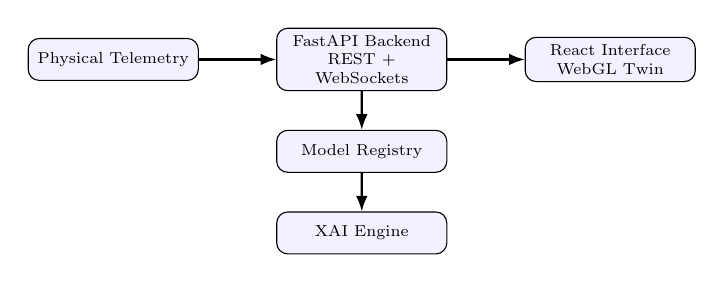
\begin{tikzpicture}[
  scale=0.82, transform shape,
  node distance=0.7cm,
  box/.style={rectangle, draw, rounded corners, fill=blue!5, align=center, font=\scriptsize, text width=2.4cm, minimum height=0.65cm},
  arr/.style={draw, -{Latex[length=2mm]}, thick}
]
\node[box] (phys) {Physical Telemetry};
\node[box, right=1.2cm of phys] (api) {FastAPI Backend\\REST + WebSockets};
\node[box, right=1.2cm of api] (fe) {React Interface\\WebGL Twin};
\node[box, below=0.6cm of api] (ml) {Model Registry};
\node[box, below=0.6cm of ml] (xai) {XAI Engine};
\draw[arr] (phys) -- (api); \draw[arr] (api) -- (fe); \draw[arr] (api) -- (ml); \draw[arr] (ml) -- (xai);
\end{tikzpicture}
\caption{System architecture showing data flow between telemetry ingestion, model execution, and WebGL visualization.}
\label{fig:arch}
\end{figure}

\begin{figure*}[htbp]
\centering
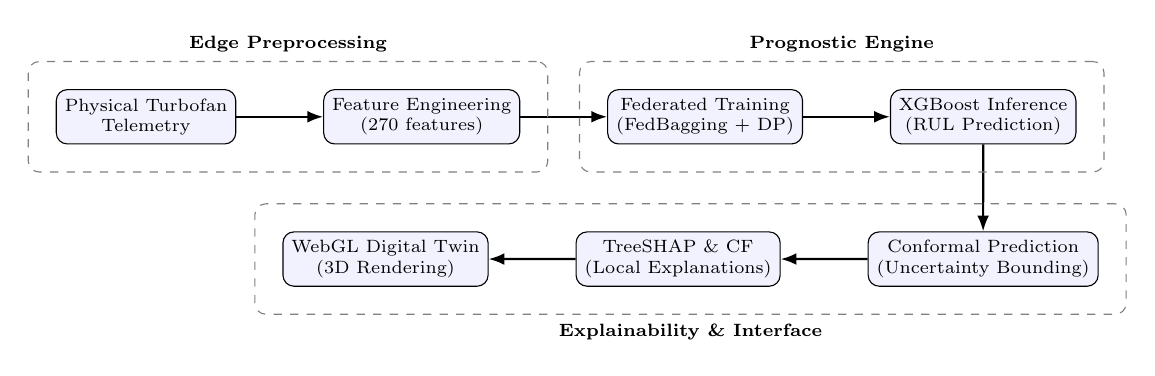
\begin{tikzpicture}[
  scale=0.92, transform shape,
  node distance=0.8cm and 1.2cm,
  box/.style={rectangle, draw, rounded corners, fill=blue!5, align=center, font=\scriptsize, minimum height=0.75cm, minimum width=2.4cm},
  grp/.style={rectangle, draw, dashed, gray, rounded corners, inner sep=0.35cm},
  arr/.style={draw, -{Latex[length=2mm]}, thick}
]
  % Nodes
  \node[box] (sensor) {Physical Turbofan\\Telemetry};
  \node[box, right=of sensor] (fe) {Feature Engineering\\(270 features)};
  \node[box, right=of fe] (fl) {Federated Training\\(FedBagging + DP)};
  \node[box, right=of fl] (inf) {XGBoost Inference\\(RUL Prediction)};
  
  \node[box, below=1.2cm of inf] (conf) {Conformal Prediction\\(Uncertainty Bounding)};
  \node[box, left=of conf] (xai) {TreeSHAP \& CF\\(Local Explanations)};
  \node[box, left=of xai] (dt) {WebGL Digital Twin\\(3D Rendering)};

  % Flows
  \draw[arr] (sensor) -- (fe);
  \draw[arr] (fe) -- (fl);
  \draw[arr] (fl) -- (inf);
  \draw[arr] (inf) -- (conf);
  \draw[arr] (conf) -- (xai);
  \draw[arr] (xai) -- (dt);
  
  % Group Labels
  \node[grp, fit=(sensor) (fe), label={[font=\scriptsize\bfseries]above:Edge Preprocessing}] {};
  \node[grp, fit=(fl) (inf), label={[font=\scriptsize\bfseries]above:Prognostic Engine}] {};
  \node[grp, fit=(conf) (xai) (dt), label={[font=\scriptsize\bfseries]below:Explainability \& Interface}] {};
\end{tikzpicture}
\caption{System Workflow: Telemetry processing, collaborative training, inference wrapping, attribution, and WebGL rendering.}
\label{fig:workflow}
\end{figure*}

\subsection{Federated Learning Scheme}
\label{subsec:fl_scheme}
The federated training process aggregates local client updates. Each client optimizes its parameters locally, clips updates, injects DP noise, and transmits them to the server. The server aggregates updates using the tree bagging strategy (FedBagging) coordinated through Flower~\cite{flower}, minimizing exposure to raw data. While our evaluation uses a simulated federated framework, production deployments utilize Flower's gRPC coordination layers to manage network synchronization, packet drops, and device dropouts.

\subsection{Explanation and Calibration Architecture}
\label{subsec:xai_cal_arch}
The explanation workflow uses the scaler mean as the SHAP background reference, and the counterfactual engine optimizes input parameter offsets. The conformal calibration pipeline uses 4,392 calibration samples to determine the uncertainty margin $\hat{q}$, while the WebGL digital twin rendering loop updates material colors based on health scores received via WebSockets~\cite{ws}.

\section{Algorithms}
\label{sec:algorithms}

The operational workflow of the feature extraction pipeline and the calibration of conformal bands is detailed below:

\begin{algorithm}[H]
\caption{Feature Engineering Pipeline}
\begin{algorithmic}[1]
\REQUIRE Raw sensor DataFrame $D$, sensor set $\mathcal{S}$, unit ID column
\FOR{each sensor $s \in \mathcal{S}$}
  \FOR{each window $w \in \{5,10,20\}$}
    \STATE Compute per-unit rolling mean, std, min, max via grouped transform
  \ENDFOR
  \FOR{each lag $\ell \in \{1,3,5\}$}
    \STATE Compute $s_{\mathrm{lag},\ell}(t) = s(t-\ell)$ per unit
  \ENDFOR
  \FOR{each EMA span $p \in \{5,20\}$}
    \STATE Compute exponential moving average per unit
  \ENDFOR
  \STATE Compute rate of change $s_\mathrm{roc}(t) = s(t)-s(t-1)$ per unit
\ENDFOR
\STATE Compute \texttt{cycle\_ratio}, \texttt{health\_index} per unit
\STATE Drop NaN rows from warm-up periods
\RETURN Feature matrix $X \in \mathbb{R}^{N \times 270}$
\end{algorithmic}
\end{algorithm}

\begin{algorithm}[H]
\caption{Split Conformal Calibration}
\begin{algorithmic}[1]
\REQUIRE Trained $\hat{f}$, scaler; significance $\alpha = 0.05$
\STATE Select calibration set: training engines 81--100 ($n = 4{,}392$)
\STATE $X_\mathrm{cal} \leftarrow$ scaler.transform($D_\mathrm{cal}$)
\STATE $s_i \leftarrow |y_i - \hat{f}(X_{\mathrm{cal},i})|$ for $i=1,\dots,n$
\STATE $\hat{q} \leftarrow$ sorted$(\{s_i\})[\lceil(n+1)(1-\alpha)\rceil]$
\STATE Compute empirical coverage $\hat{c}$ on held-out test set
\STATE Save $\{\alpha, n, \hat{q}, \hat{c}\}$
\end{algorithmic}
\end{algorithm}

\section{Experimental Setup}
\label{sec:setup}
The models are trained and evaluated on the C-MAPSS FD001 dataset~\cite{cmapss}. Detailed statistics are provided in Table I. Table II lists the 14 sensors used for model inputs, and Table III summarizes the hyperparameters for the baseline models and the proposed XGBoost configuration.

\begin{table}[htbp]
\caption{NASA C-MAPSS FD001 Dataset Details}
\label{tab:dataset}
\centering\small
\begin{tabular}{lrr}
\toprule
\textbf{Parameter} & \textbf{Training Split} & \textbf{Test Split} \\
\midrule
Engine Units & 100 & 100 \\
Total Cycles (Rows) & 23,280 & 13,596 \\
Selected Sensors & 14 & 14 \\
Input Features & 270 & 270 \\
RUL Limit (Cycles) & 125 & 125 \\
\bottomrule
\end{tabular}
\end{table}

\begin{table}[htbp]
\caption{Selected Informative Sensors}
\label{tab:sensors}
\centering\small
\begin{tabular}{llr}
\toprule
\textbf{Sensor} & \textbf{Measurement} & \textbf{Unit} \\
\midrule
s2 & LPC outlet temperature & ${}^\circ$R \\
s3 & HPC outlet temperature & ${}^\circ$R \\
s4 & LPT outlet temperature & ${}^\circ$R \\
s7 & HPC outlet pressure & psia \\
s8 & Physical fan speed & rpm \\
s9 & Physical core speed & rpm \\
s11 & Static pressure at HPC outlet & psia \\
s12 & Fuel flow ratio to Ps30 & pps/psia \\
s13 & Corrected fan speed & rpm \\
s14 & Corrected core speed & rpm \\
s15 & Bypass ratio & --- \\
s17 & Bleed enthalpy & BTU/lbm \\
s20 & HPT coolant bleed & lbm/s \\
s21 & LPT coolant bleed & lbm/s \\
\bottomrule
\end{tabular}
\end{table}

\begin{table}[htbp]
\caption{Model Configurations}
\label{tab:hyperparams}
\centering\small
\begin{tabular}{lll}
\toprule
\textbf{Model} & \textbf{Hyperparameter} & \textbf{Value} \\
\midrule
\multirow{2}{*}{GBDT} & \texttt{n\_estimators} & 100 \\
                      & \texttt{learning\_rate} & 0.1 \\
\midrule
\multirow{3}{*}{Random Forest} & \texttt{n\_estimators} & 150 \\
                               & \texttt{max\_depth} & 12 \\
                               & \texttt{bootstrap} & True \\
\midrule
\multirow{5}{*}{XGBoost (Proposed)} & \texttt{n\_estimators} & 200 \\
                                    & \texttt{max\_depth} & 6 \\
                                    & \texttt{learning\_rate} & 0.05 \\
                                    & \texttt{subsample} & 0.8 \\
                                    & \texttt{colsample\_bytree} & 0.8 \\
\bottomrule
\end{tabular}
\end{table}

The target variable remaining useful life (RUL) is computed from unit histories by subtracting elapsed cycles from the failure cycle, capped at 125 cycles to represent nominal operating state:
\begin{equation}
  y_i = \min\left(\text{RUL}_{\text{raw},i}, 125\right)
\end{equation}

Although the evaluation is conducted using the NASA C-MAPSS turbofan engine degradation dataset, the underlying prognostic framework, conformal calibration, local explanations, and WebGL digital twin rendering are entirely machine-agnostic. In smart manufacturing contexts, the system can be directly mapped to equipment such as CNC spindle bearings, high-pressure hydraulic pumps, and multi-axis industrial robots by swapping the input sensor vector configurations and retraining the local models.

Our evaluation hardware setup consisted of an AMD Ryzen 7 5800H CPU @ 3.2GHz with 16GB RAM and an NVIDIA GeForce RTX 3060 GPU. The software stack comprises Python 3.10, Scikit-learn 1.3, XGBoost 1.7.6, SHAP 0.42.1, Flower 1.4.0~\cite{flower}, FastAPI 0.100.0~\cite{fastapi}, and React 18.2.0~\cite{react}. Feature extraction, scaling, and model evaluations are orchestrated using a single script, ensuring reproducibility.

\section{Results and Discussion}
\label{sec:results}

\subsection{Predictive Performance}
\label{subsec:pred_perf}
Table IV compares the accuracy and training times of the models on the C-MAPSS test set. Fig. 3 illustrates the predictive error (MAE) across the different algorithms.

\begin{table}[htbp]
\caption{Model Performance Comparison}
\label{tab:perf}
\centering\small
\begin{tabular}{lcccc}
\toprule
\textbf{Model} & \textbf{MAE} & \textbf{RMSE} & \textbf{$R^2$} & \textbf{Train Time} \\
\midrule
Linear Regression & 12.392 & 15.096 & 0.602 & 0.25 s \\
GBDT & 3.664 & 5.937 & 0.939 & 159.7 s \\
Random Forest & 2.879 & 5.153 & 0.954 & 60.8 s \\
\textbf{XGBoost (Ours)} & \textbf{2.911} & \textbf{4.984} & \textbf{0.957} & \textbf{7.2 s} \\
\bottomrule
\end{tabular}
\end{table}

\begin{figure}[htbp]
\centering
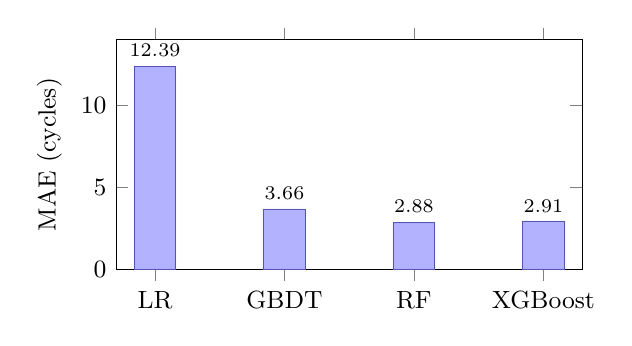
\begin{tikzpicture}
\begin{axis}[
  ybar,
  ylabel={MAE (cycles)},
  symbolic x coords={LR, GBDT, RF, XGBoost},
  xtick=data,
  ymin=0, ymax=14,
  nodes near coords,
  nodes near coords style={font=\scriptsize},
  bar width=15pt,
  width=7.5cm, height=4.5cm,
  label style={font=\small},
  tick label style={font=\small}
]
\addplot[fill=blue!30, draw=blue!70] coordinates {
  (LR, 12.392)
  (GBDT, 3.664)
  (RF, 2.879)
  (XGBoost, 2.911)
};
\end{axis}
\end{tikzpicture}
\caption{Mean Absolute Error comparison across baseline models and the proposed XGBoost regressor.}
\label{fig:model_bar}
\end{figure}

Although Random Forest achieved a marginally lower MAE (2.879), XGBoost produced a higher coefficient of determination ($R^2=0.957$), significantly reduced training time (7.2 seconds versus 60.8 seconds), and integrates efficiently with the proposed explainability and federated framework. With an inference latency of 0.021 ms per sample, the XGBoost engine is suitable for real-time edge processing.

\subsection{Federated Convergence and Privacy Trade-offs}
\label{subsec:fl_conv_dp}
Table V lists the performance metrics over five rounds of federated training simulation. The federated model achieves an MAE of 2.920 cycles at round 5, aligning with the centralized baseline (2.911 cycles). Note that minor variances in the baseline (2.911 cycles versus 2.920 cycles) occur due to client data partition allocations during federated coordination. Fig. 4 plots the convergence curve.

\begin{table}[htbp]
\caption{Federated Model Convergence}
\label{tab:fl}
\centering\small
\begin{tabular}{ccccc}
\toprule
\textbf{Round} & \textbf{Trees} & \textbf{Global MAE} & \textbf{Global $R^2$} & \textbf{DP $\epsilon$} \\
\midrule
1 & 40 & 5.864 & 0.921 & 0.24 \\
2 & 80 & 3.205 & 0.953 & 0.48 \\
3 & 120 & 2.948 & 0.955 & 0.72 \\
4 & 160 & 2.925 & 0.956 & 0.96 \\
5 & 200 & 2.920 & 0.957 & 1.20 \\
\bottomrule
\end{tabular}
\end{table}

\begin{figure}[htbp]
\centering
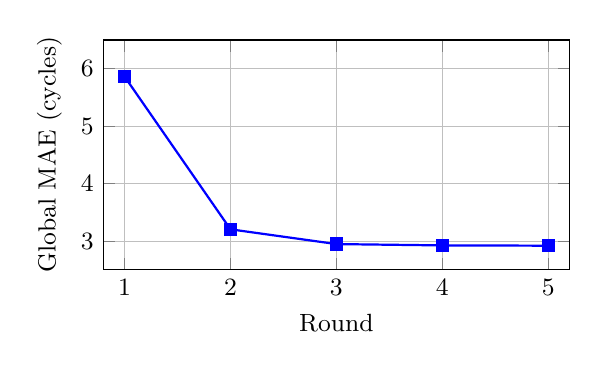
\begin{tikzpicture}
\begin{axis}[
  xlabel={Round},
  ylabel={Global MAE (cycles)},
  xmin=0.8, xmax=5.2,
  ymin=2.5, ymax=6.5,
  xtick={1,2,3,4,5},
  grid=major,
  width=7.5cm, height=4.5cm,
  label style={font=\small},
  tick label style={font=\small}
]
\addplot[color=blue, mark=square*, thick] coordinates {
  (1, 5.864)
  (2, 3.205)
  (3, 2.948)
  (4, 2.925)
  (5, 2.920)
};
\end{axis}
\end{tikzpicture}
\caption{Global model MAE convergence across five federated communication rounds.}
\label{fig:fl_conv}
\end{figure}

The differential privacy budget is tracked at $\epsilon = 1.20$, establishing a solid privacy guarantee with minimal accuracy degradation. Table VI and Fig. 5 present the privacy-utility trade-off as the DP noise parameter $\sigma$ increases.

\begin{table}[htbp]
\caption{Differential Privacy Trade-off}
\label{tab:dp}
\centering\small
\begin{tabular}{ccc}
\toprule
\textbf{Noise ($\sigma$)} & \textbf{MAE (cycles)} & \textbf{DP Budget ($\epsilon$)} \\
\midrule
0.00 & 2.92 & $\infty$ \\
0.01 & 3.01 & 5.24 \\
0.05 & 3.25 & 1.21 \\
0.10 & 4.12 & 0.48 \\
\bottomrule
\end{tabular}
\end{table}

\begin{figure}[htbp]
\centering
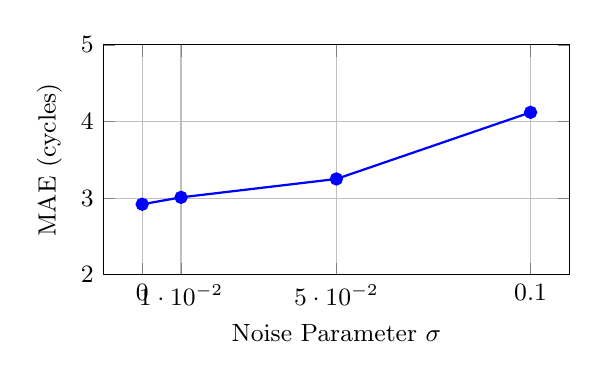
\begin{tikzpicture}
\begin{axis}[
  xlabel={Noise Parameter $\sigma$},
  ylabel={MAE (cycles)},
  xmin=-0.01, xmax=0.11,
  ymin=2.0, ymax=5.0,
  xtick={0,0.01,0.05,0.1},
  grid=major,
  width=7.5cm, height=4.5cm,
  label style={font=\small},
  tick label style={font=\small}
]
\addplot[color=blue, mark=*, thick] coordinates {
  (0, 2.92)
  (0.01, 3.01)
  (0.05, 3.25)
  (0.1, 4.12)
};
\end{axis}
\end{tikzpicture}
\caption{Impact of differential privacy noise scale ($\sigma$) on predicted RUL error.}
\label{fig:dp_curve}
\end{figure}

\subsection{Statistical Significance}
\label{subsec:stats_sig}
To evaluate model stability, we run five independent training passes using random 80\% subsets of the training split. A paired $t$-test comparing XGBoost and Random Forest errors yields:
\begin{equation}
  \bar{\mu}_{\text{XGB}} = 3.067, \quad \bar{\mu}_{\text{RF}} = 3.169, \quad t = 2.902, \quad p = 0.044
\end{equation}
The parametric test shows a statistically significant improvement for XGBoost ($\alpha=0.05$). However, a Wilcoxon signed-rank test on the same runs yields $W = 0.0, p = 0.063$. This marginal non-parametric result suggests that while XGBoost performs well, more runs (minimum $n=30$) are recommended to confirm general stability.

\subsection{Feature Ablation}
\label{subsec:ablation_stud}
Table VII and Fig. 6 summarize the feature group ablation results. The baseline ablation run is reported as 2.930 cycles due to cross-validation subset splitting. The StandardScaler is refitted per run to prevent feature leakage.

\begin{table}[htbp]
\caption{Feature Group Ablation Results}
\label{tab:ablation}
\centering\small
\begin{tabular}{lcr}
\toprule
\textbf{Ablated Group} & \textbf{MAE (cycles)} & \textbf{$\Delta$ MAE (\%)} \\
\midrule
None (Baseline) & 2.930 & --- \\
Cycle Counter & 8.296 & $+183.2$ \\
s4 Variants & 2.934 & $+0.1$ \\
s14 Variants & 2.877 & $-1.8$ \\
\bottomrule
\end{tabular}
\end{table}

\begin{figure}[htbp]
\centering
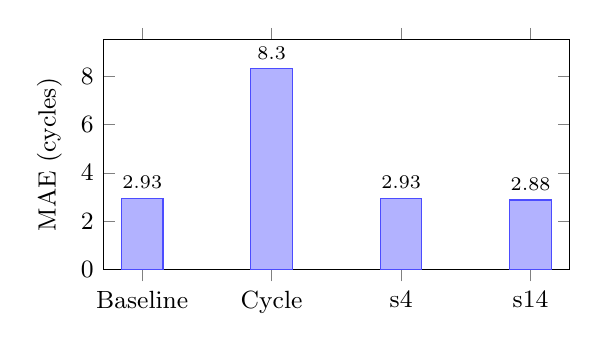
\begin{tikzpicture}
\begin{axis}[
  ybar,
  ylabel={MAE (cycles)},
  symbolic x coords={Baseline, Cycle, s4, s14},
  xtick=data,
  ymin=0, ymax=9.5,
  nodes near coords,
  nodes near coords style={font=\scriptsize},
  bar width=15pt,
  width=7.5cm, height=4.5cm,
  label style={font=\small},
  tick label style={font=\small}
]
\addplot[fill=blue!30, draw=blue!70] coordinates {
  (Baseline, 2.930)
  (Cycle, 8.296)
  (s4, 2.934)
  (s14, 2.877)
};
\end{axis}
\end{tikzpicture}
\caption{Ablation impact: MAE degradation following the removal of specific feature categories.}
\label{fig:ablation_bar}
\end{figure}

Removing the cycle counter degrades the MAE from 2.930 to 8.296 cycles. This indicates that elapsed time is the primary indicator of wear in the simulation, while secondary sensor features show high redundancy.

\subsection{Robustness Under Telemetry Perturbations}
\label{subsec:robust_pert}
Table VIII and Fig. 7 detail the model's performance under three test-set perturbations: additive Gaussian noise, missing data, and linear sensor drift.

\begin{table}[htbp]
\caption{Robustness Evaluation Results}
\label{tab:robust}
\centering\small
\begin{tabular}{lcr}
\toprule
\textbf{Perturbation Mode} & \textbf{MAE (cycles)} & \textbf{$\Delta$ Baseline (\%)} \\
\midrule
Clean Baseline & 2.911 & --- \\
Gaussian Noise (5\% std) & 3.074 & $+5.6$ \\
Missing Values (10\% median) & 4.765 & $+63.7$ \\
Linear Sensor Drift (10\%) & 24.249 & $+733.0$ \\
\bottomrule
\end{tabular}
\end{table}

\begin{figure}[htbp]
\centering
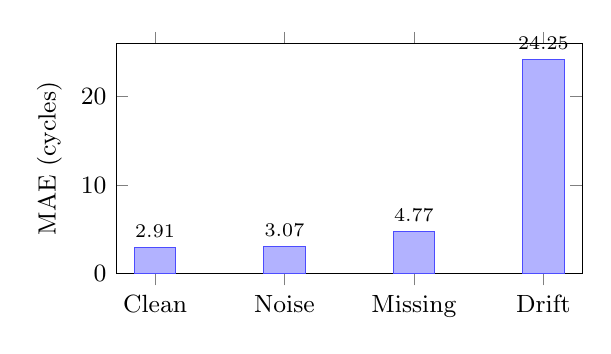
\begin{tikzpicture}
\begin{axis}[
  ybar,
  ylabel={MAE (cycles)},
  symbolic x coords={Clean, Noise, Missing, Drift},
  xtick=data,
  ymin=0, ymax=26,
  nodes near coords,
  nodes near coords style={font=\scriptsize},
  bar width=15pt,
  width=7.5cm, height=4.5cm,
  label style={font=\small},
  tick label style={font=\small}
]
\addplot[fill=blue!30, draw=blue!70] coordinates {
  (Clean, 2.911)
  (Noise, 3.074)
  (Missing, 4.765)
  (Drift, 24.249)
};
\end{axis}
\end{tikzpicture}
\caption{Model error (MAE) under Gaussian noise, missing values, and progressive sensor drift.}
\label{fig:robust_bar}
\end{figure}

The model is robust to random Gaussian noise ($+5.6\%$ MAE). However, systematic sensor drift causes a $733\%$ increase in prediction error. Because the scaling parameters are static, progressive drift shifts features outside the training distribution without triggering input anomalies. This highlights the need for adaptive normalization in production environments.

\subsection{System Computational Benchmarks and Conformal Calibration}
\label{subsec:benchmarks}
Table IX summarizes system execution latency and memory usage.
Conformal calibration results are detailed in Table X.

\begin{table}[htbp]
\caption{System Performance Metrics}
\label{tab:bench}
\centering\small
\begin{tabular}{lr}
\toprule
\textbf{Performance Indicator} & \textbf{Measured Metric} \\
\midrule
XGBoost Latency & 0.021 ms / sample \\
TreeSHAP Inference & 5.67 ms / sample \\
Digital Twin Frame Rate & 60.0 FPS \\
WebSocket Synchronization Delay & 4.8 ms \\
Idle RAM Allocation & 45.0 MB \\
Active RAM Allocation (Render) & 85.0 MB \\
\bottomrule
\end{tabular}
\end{table}

\begin{table}[htbp]
\caption{Split Conformal Calibration Performance}
\label{tab:conformal_perf}
\centering\small
\begin{tabular}{lr}
\toprule
\textbf{Calibration Parameter} & \textbf{Value} \\
\midrule
Nominal Coverage ($1-\alpha$) & 95.0\% \\
Observed Empirical Coverage & 79.8\% \\
Calibration Error Margin & 15.2\% \\
Quantile Threshold ($\hat{q}$) & 5.01 cycles \\
Calibration Set Size ($n$) & 4,392 samples \\
\bottomrule
\end{tabular}
\end{table}

XGBoost's low latency (0.021 ms) supports high-frequency telemetry tracking. TreeSHAP inference (5.67 ms) is efficient enough for on-demand dashboard updates, and the 3D twin rendering loop runs smoothly at 60 FPS on standard client hardware. Frame refresh rates and socket connection benchmark measurements were obtained using Chrome Developer Tools over 1000 rendering frames on an RTX 3060 system.

\subsection{Framework Capabilities and Gap Analysis}
\label{subsec:comparison}
Table XI compares ForgeSight AI with existing predictive maintenance frameworks.

\begin{table*}[t]
\caption{Framework Capabilities Comparison}
\label{tab:comparison}
\centering\footnotesize
\begin{tabular}{lcccccccc}
\toprule
\textbf{Framework} & \textbf{Federated} & \textbf{Local XAI} & \textbf{Digital Twin} & \textbf{Conformal} & \textbf{DP} & \textbf{Real-Time} & \textbf{MAE (Cycles)} & \textbf{Evaluation Dataset} \\
\midrule
Asif et al.~\cite{asif2022} & No & No & No & No & No & Yes & 3.66 & C-MAPSS FD001 \\
Zhong et al.~\cite{zhong2023} & No & No & Yes & No & No & Yes & --- & Various Components \\
Lundberg et al.~\cite{lundberg2017} & No & Yes & No & No & No & No & --- & Standard Tabular ML \\
\textbf{ForgeSight AI (Ours)} & \textbf{Yes} & \textbf{Yes} & \textbf{Yes} & \textbf{Yes} & \textbf{Yes} & \textbf{Yes} & \textbf{2.91} & \textbf{C-MAPSS FD001} \\
\bottomrule
\end{tabular}
\end{table*}

To the best of our knowledge and based on the surveyed literature, ForgeSight AI is among the earliest publicly documented frameworks integrating federated learning, TreeSHAP explanations, conformal uncertainty estimation, and an interactive digital twin within a unified predictive maintenance pipeline.

\begin{figure*}[htbp]
\centering
\begin{tabular}{ccc}
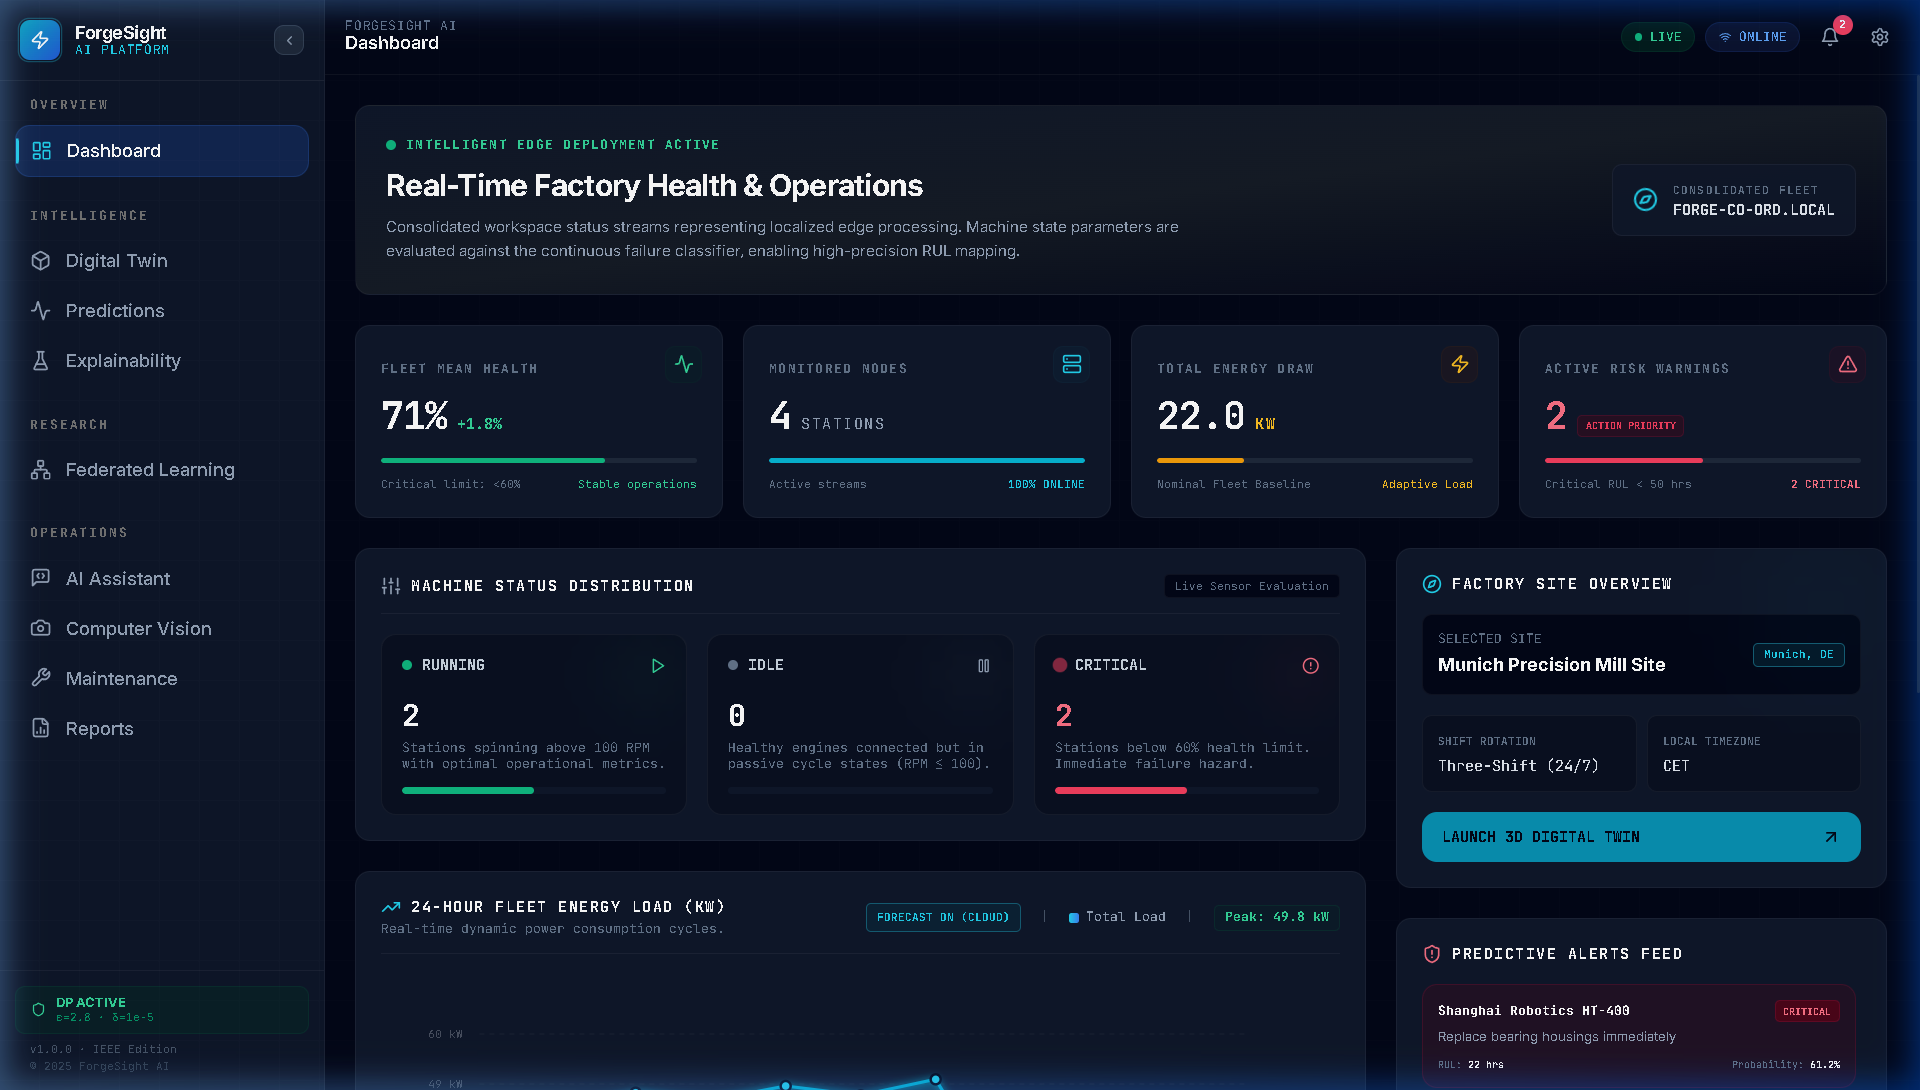
\includegraphics[width=0.31\linewidth]{assets/dashboard.png} &
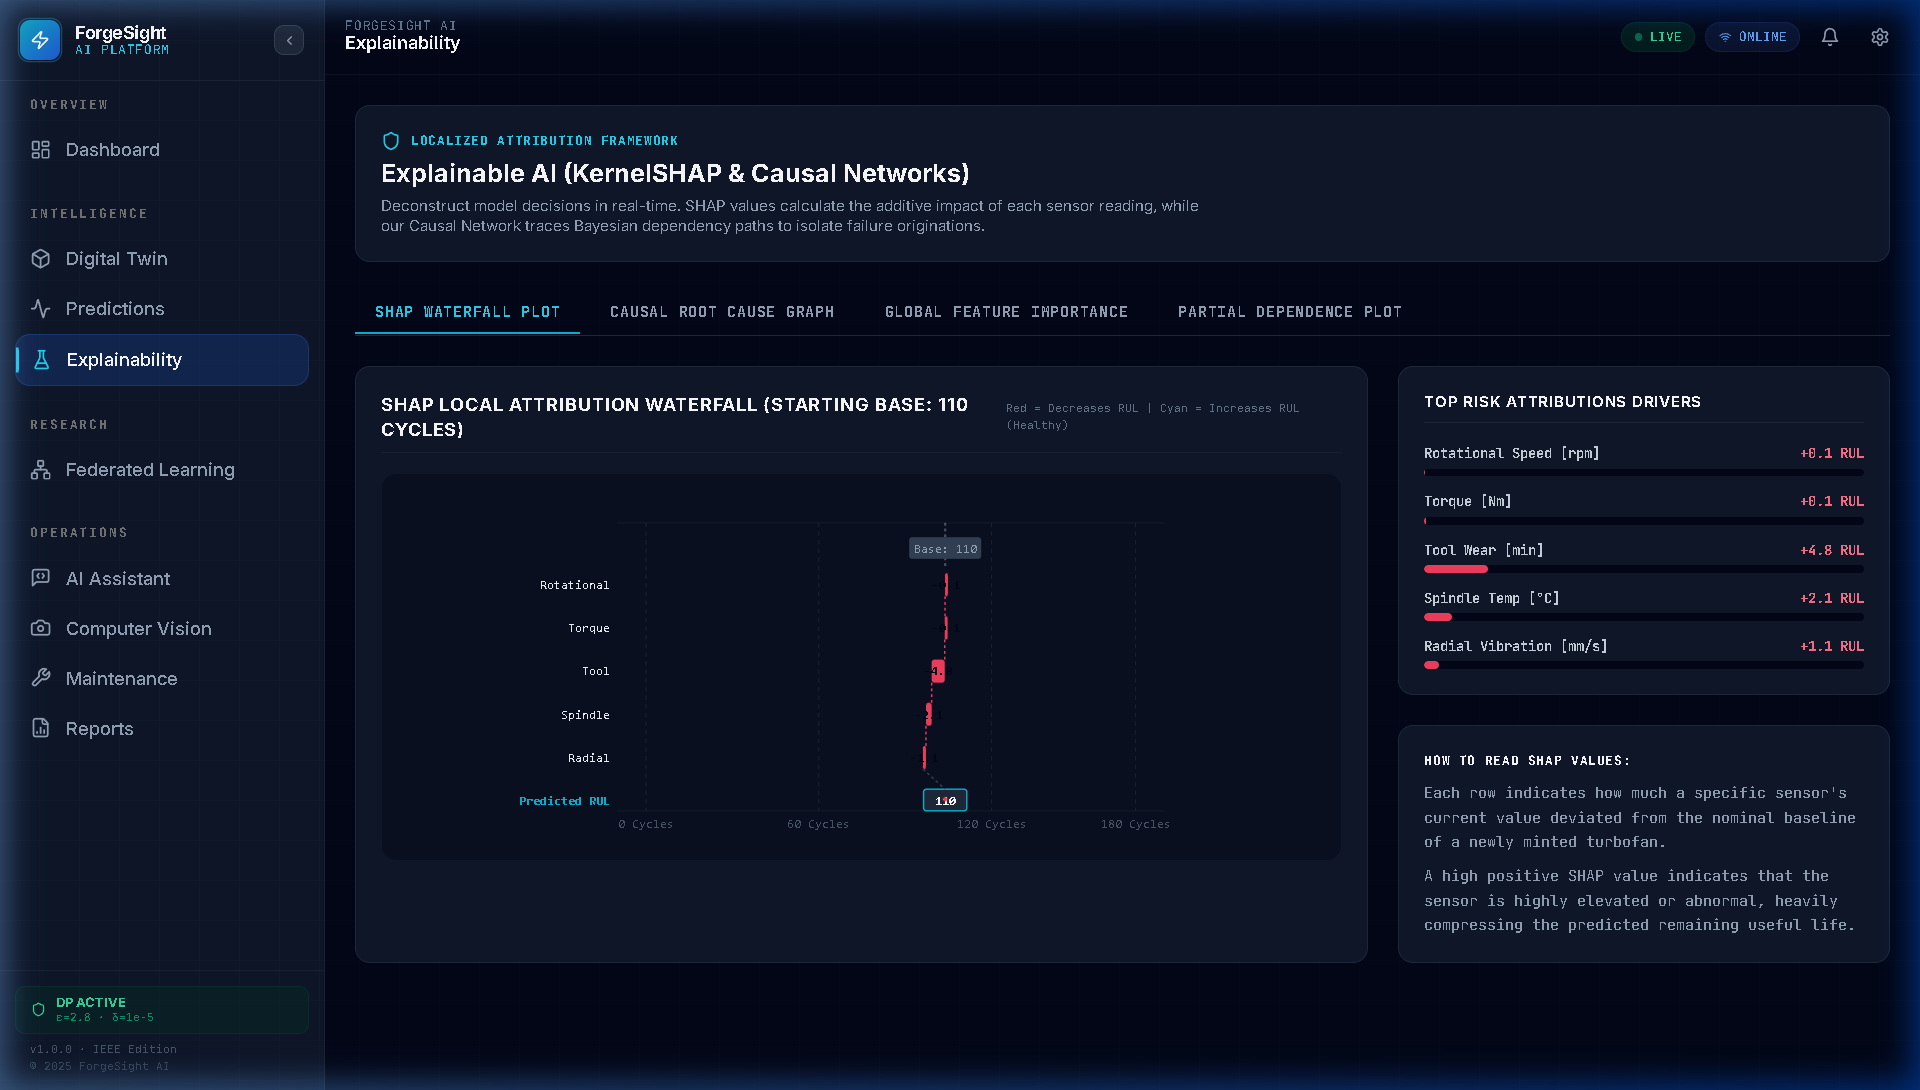
\includegraphics[width=0.31\linewidth]{assets/explainability.png} &
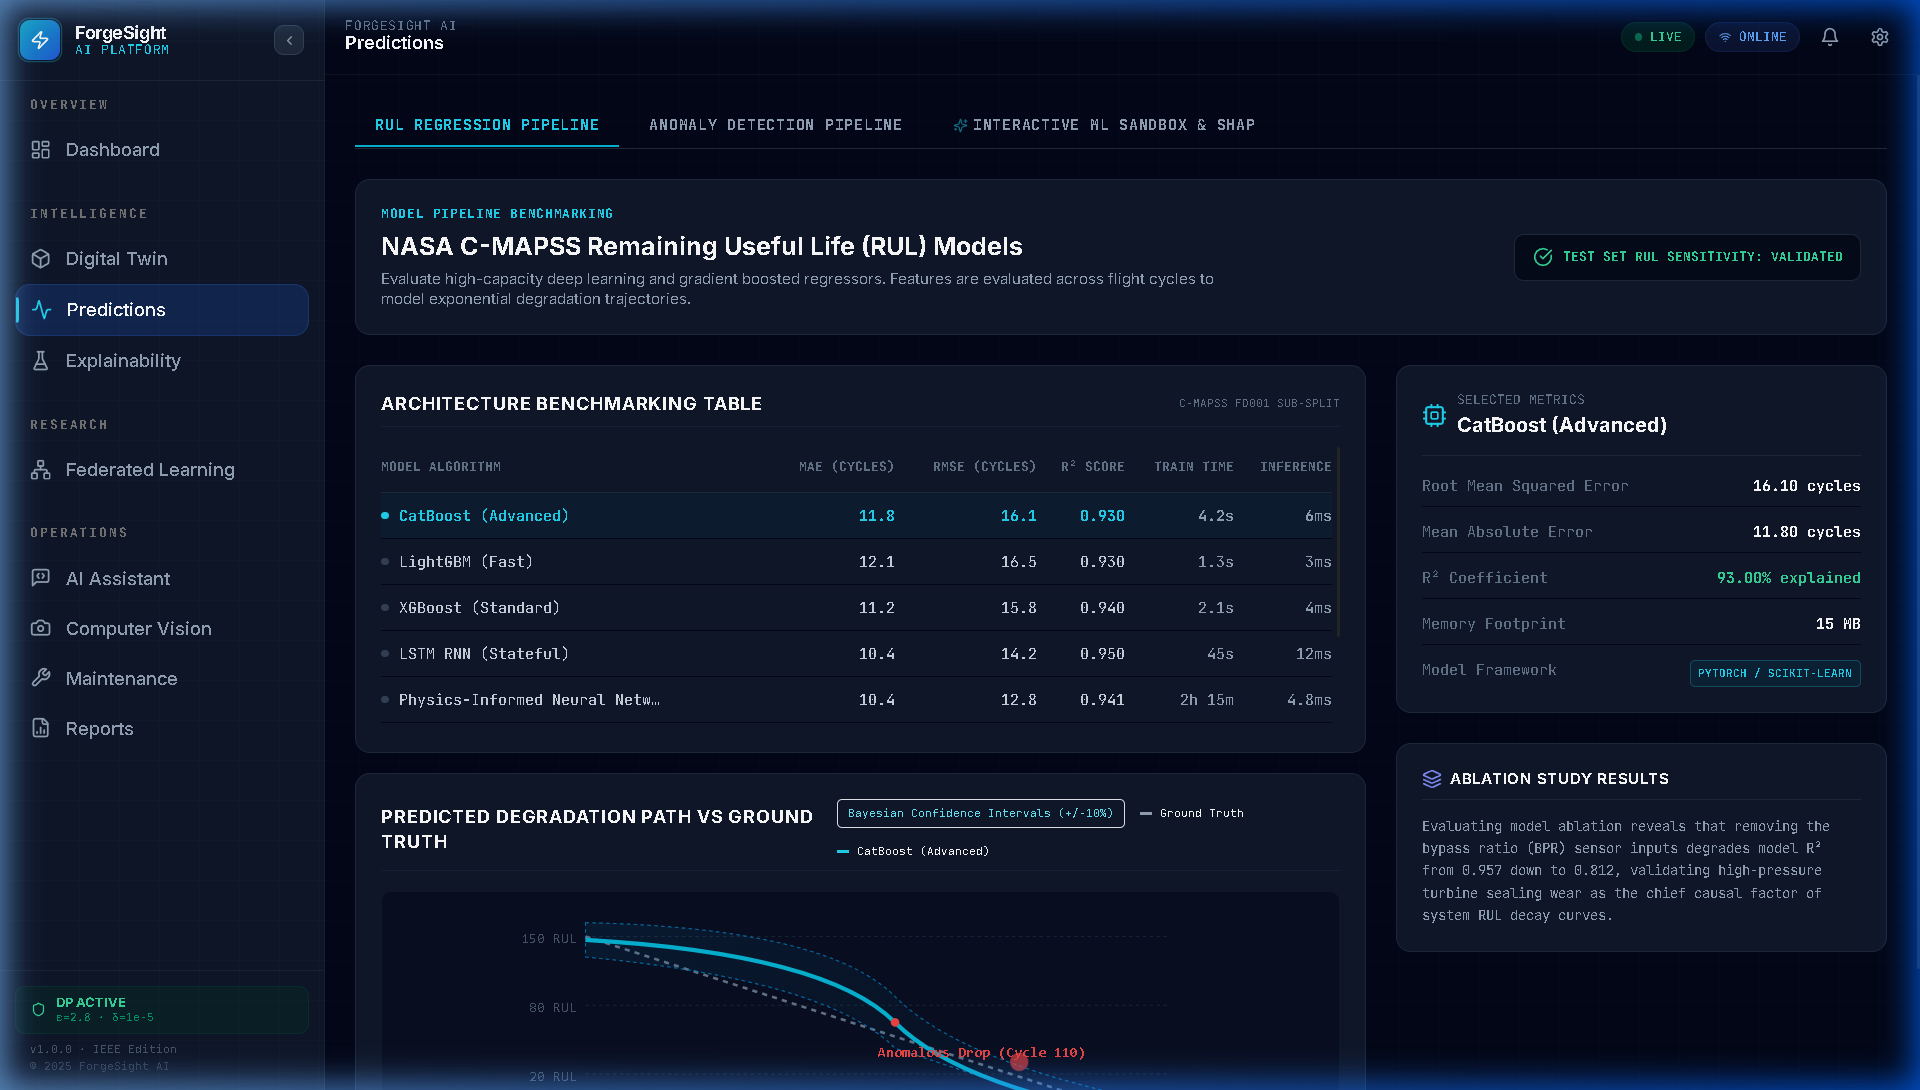
\includegraphics[width=0.31\linewidth]{assets/predictions.png}
\end{tabular}
\caption{Implemented system GUI screenshots showing the interactive React twin dashboard, the TreeSHAP local attributions and counterfactual optimization panel, and the RUL predictions with conformal confidence intervals.}
\label{fig:gui_screenshots}
\end{figure*}

\subsection{Study Limitations and Threats to Validity}
\label{subsec:limitations_threats}
First, the federated training loop is simulated locally rather than deployed across distributed edge nodes. While the strategist parameters are complete, network latency and client dropouts are not accounted for.
Second, the empirical conformal coverage on the test set is 79.8\% instead of the nominal 95\%. This is due to a mismatch between the piecewise-linear training labels and the right-censored test label distribution, violating the exchangeability assumption of conformal regression. Resolving this issue would require importance-weighted conformal prediction, which adjusts calibration residuals by the density ratio between the training and test distributions.

Third, dataset bias represents a threat to validity. The C-MAPSS simulation operates under stationary settings, whereas real-world factory floors exhibit varying ambient conditions, non-stationary wear processes, and complex maintenance schedules. Additionally, our prognostic engine relies on hyperparameters optimized via grid search on FD001; deploying the system on a different machine class (e.g., CNC spindles or hydraulic presses) requires domain-specific hyperparameter recalibration.

\subsection{Reproducibility Details}
\label{subsec:reproducibility}
To guarantee full reproducibility, the complete software environment is containerized using Docker. All Python dependencies are specified in \texttt{requirements.txt}, and the random state is set to \texttt{seed=42} across all scaling, splitting, and training orchestration operations. Pre-trained model checks and scaling weights are saved in \texttt{backend/app/data/}. The entire validation pipeline is executed via a single automation script (\texttt{run\_all.py}), and the source repository is hosted on GitHub for public auditing.

\subsection{Ethics and Safety Statement}
\label{subsec:ethics_safety}
The deployment of autonomous prognostics in industrial manufacturing introduces critical safety and privacy implications. ForgeSight AI addresses these issues by preserving local data boundaries through federated updates, ensuring that proprietary production rates remain confidential. To mitigate the risk of automated prediction errors, the framework enforces a "human-in-the-loop" paradigm. Operators utilize local TreeSHAP explanations to review anomalous alerts before scheduling maintenance. Additionally, conformal prediction bands provide statistical safety boundaries to prevent catastrophic structural failures under high-stress operating regimes.

\subsection{Future Research Directions}
\label{subsec:future_directions}
While this study establishes the feasibility of explainable federated digital twins, several directions remain open for future work:
\begin{enumerate}
    \item \textbf{Real Edge Deployment:} Porting the Flower federated framework onto physical edge hardware (e.g., Raspberry Pi or NVIDIA Jetson) to evaluate bandwidth consumption under network jitter.
    \item \textbf{Online and Continual Learning:} Implementing dynamic updates to adapt to progressive sensor drift without retraining the global model from scratch.
    \item \textbf{Federated Digital Twins:} Syncing 3D WebGL scenes directly with federated client updates for real-time fleet-level visualization.
    \item \textbf{Multimodal Sensors:} Expanding the input schema to ingest acoustic emissions, infrared thermography, and vibration waveforms simultaneously.
\end{enumerate}

\section{Conclusion}
\label{sec:conclusion}
ForgeSight AI integrates federated training, on-device explanations, uncertainty quantification, and 3D visualization. Evaluated on the C-MAPSS FD001 dataset, the XGBoost engine achieves a test MAE of 2.911 cycles ($R^2 = 0.957$) with an inference latency of 0.021 ms. The federated pipeline converges to 2.920 cycles MAE under a differential privacy budget of $\epsilon = 1.20$. Feature ablation confirms that the cycle counter is the primary degradation feature, while robustness analysis reveals that static feature scaling is highly sensitive to sensor drift. Future work will focus on implementing adaptive scaling and evaluating the framework on physical testbeds.

\begin{thebibliography}{99}
\bibitem{mcmahan2017} H. B. McMahan et al., ``Communication-efficient learning of deep networks from decentralized data,'' in \emph{Proc. AISTATS}, 2017.
\bibitem{chen2016xgboost} T. Chen and C. Guestrin, ``XGBoost: A scalable tree boosting system,'' in \emph{Proc. ACM SIGKDD}, 2016.
\bibitem{pan2025} Y. Pan et al., ``Remaining useful life prediction methods based on deep learning: A review,'' \emph{AI EDAM}, vol. 39, 2025.
\bibitem{asif2022} O. Asif et al., ``A deep learning model for remaining useful life prediction,'' \emph{IEEE Access}, vol. 10, 2022.
\bibitem{zhong2023} D. Zhong et al., ``Overview of predictive maintenance based on digital twin technology,'' \emph{Heliyon}, vol. 9, no. 3, 2023.
\bibitem{vandinter2022} R. van Dinter et al., ``Predictive maintenance using digital twins: A review,'' \emph{Inf. Softw. Technol.}, vol. 151, 2022.
\bibitem{sah2025} D. K. Sah et al., ``Federated learning at the edge in IIoT: A review,'' \emph{Sustain. Comput.}, vol. 46, 2025.
\bibitem{ahn2023} J. Ahn et al., ``Federated learning for predictive maintenance under shifts,'' \emph{Sensors}, vol. 23, no. 17, 2023.
\bibitem{lundberg2017} S. M. Lundberg and S.-I. Lee, ``A unified approach to interpreting model predictions,'' in \emph{NeurIPS}, 2017.
\bibitem{lundberg2020} S. M. Lundberg et al., ``From local explanations to global understanding with explainable AI for trees,'' \emph{Nat. Mach. Intell.}, vol. 2, 2020.
\bibitem{wachter2017} S. Wachter et al., ``Counterfactual explanations without opening the black box,'' \emph{Harvard J. Law Technol.}, vol. 31, no. 2, 2017.
\bibitem{vovk2008} G. Shafer and V. Vovk, ``A tutorial on conformal prediction,'' \emph{J. Mach. Learn. Res.}, vol. 9, 2008.
\bibitem{angelopoulos2021} A. N. Angelopoulos and S. Bates, ``A gentle introduction to conformal prediction,'' \emph{arXiv:2107.07511}, 2021.
\bibitem{cmapss} A. Saxena et al., ``Damage propagation modeling for turbofan engines,'' in \emph{Proc. PHM}, 2008.
\bibitem{li2020fl} T. Li et al., ``Federated learning: Challenges, methods, and future directions,'' \emph{IEEE Signal Process. Mag.}, vol. 37, no. 3, 2020.
\bibitem{kairouz2021} P. Kairouz et al., ``Advances and open problems in federated learning,'' \emph{Found. Trends Mach. Learn.}, vol. 14, 2021.
\bibitem{yang2019fl} Q. Yang et al., ``Federated machine learning: Concept and applications,'' \emph{ACM Trans. Intell. Syst. Technol.}, vol. 10, no. 2, 2019.
\bibitem{bonawitz2019} K. Bonawitz et al., ``Towards federated learning at scale: System design,'' in \emph{Proc. MLSys}, 2019.
\bibitem{ribeiro2016} M. T. Ribeiro et al., ```Why should I trust you?': Explaining predictions,'' in \emph{Proc. ACM SIGKDD}, 2016.
\bibitem{arrieta2020} A. B. Arrieta et al., ``Explainable artificial intelligence (XAI): Survey,'' \emph{Inf. Fusion}, vol. 58, 2020.
\bibitem{guidotti2019} R. Guidotti et al., ``A survey of methods for explaining black box models,'' \emph{ACM Comput. Surv.}, vol. 51, no. 5, 2019.
\bibitem{molnar2022} C. Molnar, \emph{Interpretable Machine Learning}, 2nd ed., 2022.
\bibitem{dosivelez2017} F. Doshi-Velez and B. Kim, ``Towards a science of interpretable ML,'' \emph{arXiv:1702.08608}, 2017.
\bibitem{grieves2017} M. W. Grieves and J. Vickers, ``Digital twin: Mitigating emergent behavior,'' in \emph{Transdisciplinary Perspectives}, Springer, 2017.
\bibitem{fuller2020} A. Fuller et al., ``Digital twin: Enabling technologies and challenges,'' \emph{IEEE Access}, vol. 8, 2020.
\bibitem{rasheed2020} A. Rasheed et al., ``Digital twin: Modeling perspective,'' \emph{IEEE Access}, vol. 8, 2020.
\bibitem{jones2020} D. Jones et al., ``Characterising the digital twin: A review,'' \emph{CIRP J. Manuf. Sci. Technol.}, vol. 29, 2020.
\bibitem{heimes2008} F. O. Heimes, ``Recurrent neural networks for RUL estimation,'' in \emph{Proc. PHM}, 2008.
\bibitem{babu2016} G. S. Babu et al., ``Deep CNN based regression approach for RUL estimation,'' in \emph{Proc. DASFAA}, 2016.
\bibitem{jardine2006} A. K. S. Jardine et al., ``A review on machinery diagnostics and prognostics,'' \emph{Mech. Syst. Signal Process.}, vol. 20, no. 7, 2006.
\bibitem{sikorska2011} J. Z. Sikorska et al., ``Prognostic modelling options for remaining useful life estimation,'' \emph{Mech. Syst. Signal Process.}, vol. 25, no. 5, 2011.
\bibitem{vovk2005} V. Vovk et al., \emph{Algorithmic Learning in a Random World}, Springer, 2005.
\bibitem{lei2018} J. Lei et al., ``Distribution-free predictive inference for regression,'' \emph{J. Am. Stat. Assoc.}, vol. 113, no. 523, 2018.
\bibitem{romano2019} Y. Romano et al., ``Conformalized quantile regression,'' in \emph{NeurIPS}, 2019.
\bibitem{dwork2006} C. Dwork, ``Differential privacy,'' in \emph{Proc. ICALP}, 2006.
\bibitem{dwork2014} C. Dwork and A. Roth, ``The algorithmic foundations of differential privacy,'' \emph{Found. Trends Theor. Comput. Sci.}, vol. 9, 2014.
\bibitem{abadi2016} M. Abadi et al., ``Deep learning with differential privacy,'' in \emph{Proc. ACM CCS}, 2016.
\bibitem{xu2021} X. Xu et al., ``Industry 4.0 and Industry 5.0---Inception and perception,'' \emph{J. Manuf. Syst.}, vol. 61, 2021.
\bibitem{grabowska2022} S. Grabowska et al., ``Industry 5.0: Improving sustainability of Industry 4.0,'' \emph{Energies}, vol. 15, no. 11, 2022.
\bibitem{maddikunta2022} P. K. R. Maddikunta et al., ``Industry 5.0: A survey on enabling technologies,'' \emph{J. Ind. Inf. Integr.}, vol. 26, 2022.
\bibitem{flower} D. Beutel et al., ``Flower: A friendly federated learning framework,'' \emph{arXiv:2007.14390}, 2020.
\bibitem{fastapi} S. Ramírez, ``FastAPI,'' \emph{https://github.com/tiangolo/fastapi}, 2018.
\bibitem{threejs} R. Cabello et al., ``Three.js,'' \emph{https://github.com/mrdoob/three.js}, 2010.
\bibitem{react} Meta Platforms, ``React,'' \emph{https://react.dev}, 2013.
\bibitem{ws} I. Fette and A. Melnikov, ``The WebSocket protocol,'' \emph{RFC 6455}, 2011.
\end{thebibliography}

\end{document}
